% Title and certificate pages are omitted as requested.
\pagenumbering{roman}
\fancypagestyle{frontmatter}{\fancyhf{}\fancyfoot[C]{\textit{\thepage}}\renewcommand{\headrulewidth}{0pt}\renewcommand{\footrulewidth}{0pt}}
\fancypagestyle{plain}{\fancyhf{}\fancyfoot[C]{\textit{\thepage}}\renewcommand{\headrulewidth}{0pt}\renewcommand{\footrulewidth}{0pt}}
\renewcommand{\cftlottitlefont}{\hfill\bfseries\fontsize{16}{20}\selectfont}\renewcommand{\cftafterlottitle}{\hfill}
\renewcommand{\cftloftitlefont}{\hfill\bfseries\fontsize{16}{20}\selectfont}\renewcommand{\cftafterloftitle}{\hfill}
\pagestyle{frontmatter}
\titleformat{\chapter}[block]{\bfseries\fontsize{16}{20}\selectfont\centering}{}{0pt}{}
\renewcommand{\cfttoctitlefont}{\hfill\bfseries\fontsize{16}{20}\selectfont}\renewcommand{\cftaftertoctitle}{\hfill}

\chapter*{Acknowledgement}
\addcontentsline{toc}{chapter}{Acknowledgement}
I express my sincere gratitude to the management of Mar Athanasius
College of Engineering, Kothamangalam, for providing the academic
environment and facilities needed to undertake this mini project. The
project gave me an opportunity to apply my learning in data science,
machine learning, software development, and responsible data analysis.

I extend my heartfelt appreciation to my project guide, Dr.Manu John,
Department of Computer Applications, for his valuable guidance,
technical suggestions, and encouragement throughout the planning,
development, and documentation of the AI Forensic Insider Risk Review
System. His feedback helped me refine the project and present its
methods and limitations more clearly.

I am sincerely grateful to Dr.Sonia Abraham, Head of the Department of
Computer Applications, for her encouragement and support. I also thank
the project coordinators, faculty members, and staff of the department
for their guidance and assistance during the project.

I acknowledge the creators of the CERT Insider Threat Test Dataset and
the developers and maintainers of the open-source tools used in this
work. Their contributions supported the study of synthetic activity
records and the implementation of the data-processing, modelling, and
dashboard components.

Finally, I express my heartfelt gratitude to my parents, family
members, and friends for their patience, encouragement, and support. I
also thank everyone who contributed directly or indirectly to the
completion of this mini project and its report.

\chapter*{Abstract}
\addcontentsline{toc}{chapter}{Abstract}
Insider-risk review is difficult because potentially relevant activity
is distributed across multiple systems, the number of routine events is
large, and known incident examples are rare. This mini project presents
Forensio, a local-first review system that aggregates logon, removable
device, file, email, and web activity into employee-day features and
uses four different model perspectives to prioritize records for human
inspection. The implementation combines a Python data and scoring
pipeline, a FastAPI service, and a React review dashboard; a Streamlit
interface remains available as an alternative.

The model-development study uses the CERT r4.2 synthetic insider-threat
dataset. Its saved labelled table contains 330,452 employee-days for
1,000 synthetic users, of which 1,364 employee-days overlap a listed
incident interval under the project's labeling rule. Activity events
are cleaned and aggregated by user and calendar day. A grouped
train/validation/test design keeps users disjoint between partitions.
The notebook compares Logistic Regression, Decision Tree, Random
Forest, and Isolation Forest, selects variants and a review capacity
using validation data, and evaluates the selected operating point on a
held-out test partition. In the saved one-percent review-capacity
evaluation, the Random Forest has precision 0.144, recall 0.329, F1
0.200, and average precision 0.158. The dashboard separately combines
within-dataset percentile ranks and applies an employee-level queue
rule.

The system is a research and demonstration prototype, not an
investigative finding engine. A high rank is neither a probability nor
evidence of misconduct. The dataset is synthetic, labels are
incident-window proxies, queue rules are relative to a selected
dataset, and the current features do not model employee roles,
schedules, or context. Human review, corroborating evidence, access
controls, and documented governance are therefore essential before any
operational use.

\renewcommand{\listtablename}{List of tables}
\listoftables

\renewcommand{\listfigurename}{List of figures}
\listoffigures

\clearpage
\pagestyle{frontmatter}
\tableofcontents

\clearpage
\pagenumbering{arabic}
\setcounter{page}{1}
\titleformat{\chapter}[hang]{\bfseries\fontsize{16}{20}\selectfont}{\thechapter.}{0.65em}{}
\fancypagestyle{plain}{\fancyhf{}\fancyhead[R]{\small\projecttitle}\fancyfoot[L]{\small\department}\fancyfoot[R]{\thepage}\renewcommand{\headrulewidth}{0.4pt}\renewcommand{\footrulewidth}{0.4pt}}
\pagestyle{reportstyle}
\onehalfspacing

\chapter{Introduction}
\label{chap:introduction}

\section{Background}
Modern organisations generate activity records through identity
providers, endpoints, file services, email systems, and web gateways.
These records are useful for security operations, but their volume and
fragmentation make manual review difficult. A security analyst may
need to correlate a sequence of events across several sources before
deciding whether it warrants escalation. The challenge is not simply
to detect a single unusual event; it is to organise context in a way
that supports a careful and reproducible investigation.

Insider-risk analysis concerns activity associated with trusted
accounts and authorised access. A meaningful review must distinguish
between a statistical signal and a conclusion about a person.
Legitimate work can produce unusual activity, while harmful activity
may resemble normal operations. Differences in job role, work schedule,
travel, project deadlines, and system configuration can all affect the
observed event pattern. For that reason, a decision-support tool should
make its inputs and ranking logic understandable and should preserve
human authority over all consequential decisions.

This project implements a prototype called Forensio. It transforms
five activity logs into employee-day counts, scores those feature rows
using four model families, and displays a ranked review queue. It is
designed to demonstrate a technical workflow on the CERT r4.2
synthetic dataset. It is not a production surveillance platform, does
not inspect message or file content, and does not establish intent.

\section{Problem statement}
The project addresses the following bounded problem: given a local
folder containing the five supported activity CSV files and a
previously trained model bundle, produce an employee-day and
employee-level ranking that helps an analyst decide which records to
review first. The system must integrate disparate sources, handle
large CSV files with bounded-memory processing, apply the same feature
contract used in training, expose clear model context, and avoid
presenting a score as proof.

The study also evaluates whether a set of supervised and unsupervised
models can rank synthetic incident-window employee-days above other
days when users are kept separate across development and test
partitions. A low base rate makes accuracy alone unsuitable as the
primary measure. The study therefore reports average precision and
capacity-based precision, recall, and F1 alongside the confusion
counts.

\section{Objectives of the project}
The objectives are to:
\begin{enumerate}
  \item examine the supported activity data and its quality;
  \item build a repeatable employee-day aggregation and labeling
  workflow;
  \item compare four distinct model families under user-grouped
  evaluation;
  \item build a local scoring service that reuses the trained feature
  schema;
  \item create a dashboard for selecting data, following analysis
  progress, and reviewing ranked employees and activity details;
  \item document evaluation limits, privacy considerations, and
  responsible-use controls.
\end{enumerate}

\section{Scope of the project}
The project scope includes synthetic logon, device, file, email, and
HTTP event records; aggregation at one calendar day per user; the
feature columns persisted with the trained bundle; offline model
evaluation; local scoring; and a human-readable review interface.
Optional employee-name lookup files are supported by the local scoring
code, but names are not required for model input.

The current scope excludes live collection agents, enterprise identity
integrations, cross-organisation model transfer, streaming analysis,
automated disciplinary decisions, legal attribution, message-body or
file-content inspection, calibrated probability estimates, and
production authentication or role-based access control. A dashboard
rank is relative to the data batch being scored. The offline
employee-day test results do not validate the dashboard's
employee-level status rule.

\section{Project domain and technology stack}
The project combines data engineering, applied machine learning,
information visualization, and digital-forensics workflow concepts.
Python and pandas perform input handling and aggregation;
scikit-learn supplies estimators and metrics; joblib persists the
model bundle; FastAPI exposes a local HTTP interface; and React,
JavaScript, Vite, and CSS provide the browser dashboard. Streamlit is
retained as an alternative interface. CSV files are used for both
inputs and result exports; the prototype does not require a database.

\begin{table}[H]
\centering
\tablefont
\caption{Project components and their responsibilities}
\label{tab:technology-stack}
\begin{tabularx}{\textwidth}{|p{0.24\textwidth}|p{0.25\textwidth}|Y|}
\hline
\textbf{Component} & \textbf{Technology} & \textbf{Responsibility}\\\hline
Data preparation & Python, pandas, NumPy & Clean activity records, aggregate features, and align model columns.\\\hline
Model development & scikit-learn & Fit and evaluate supervised and unsupervised estimators.\\\hline
Model persistence & joblib & Store estimators and the feature-column contract for local reuse.\\\hline
Service layer & FastAPI, Pydantic & Validate requests, manage analysis endpoints, and return JSON results.\\\hline
Web interface & React, Vite, CSS & Select log folders, display progress, search and filter the review queue.\\\hline
Alternative interface & Streamlit & Provide a Python-only local demonstration path.\\\hline
Input and outputs & CSV & Interchange activity logs, scores, and report tables.\\\hline
\end{tabularx}
\end{table}

\section{Organisation of the report}
Chapter 2 reviews insider-risk analytics and relevant evaluation
principles. Chapter 3 describes the dataset, preprocessing,
visualization, algorithms, pipeline, feasibility, and operating
environment. Chapter 4 presents model construction, software
architecture, requirements, data design, and interface design.
Chapter 5 reports the saved model evaluation and discusses its limits.
Chapter 6 describes the local deployment and analyst workflow.
Chapter 7 summarises the repository history. Chapters 8 and 9 give the
conclusions and future work. Chapter 10 contains reproducibility
information, requirements, test cases, data definitions, responsible
use guidance, and source listings. Chapter 11 provides references.

\chapter{Supporting literature}
\label{chap:literature}

\section{Literature review}
Insider-risk detection is difficult because legitimate and risky
activities can share the same systems and permissions. Research
therefore examines both user behaviour and the context needed to
interpret it, rather than treating a model score as proof of intent.
The CERT Insider Threat Test Dataset provides synthetic scenarios and
activity records for repeatable experiments \cite{cert}. Synthetic
data avoids exposing real employee records during development, but
results on one generated release do not establish performance in a
real organisation.

Rahman, Al Naeem, and Abubakar study unintentional-insider readiness
using CERT r4.2 activity data and a nonlinear autoregressive model with
exogenous inputs (NARX). They describe access, motivation, and action
as dimensions of insider behaviour and report a best-partition
\(R^2\) value of 0.97 for their proposed formulation
\cite{rahman2022unintentional}. This work is relevant because it
explicitly considers unintentional rather than exclusively malicious
behaviour. Its target formulation and reported statistic differ from
the employee-day classification and review-capacity metrics used in
this project, so the figures should not be compared as if they measured
the same task.

Al-Shehari et al. investigate an anomaly-based Isolation Forest model
for the class-imbalance problem in insider-threat data, using the CERT
benchmark and varying the model's contamination setting. They report
98\% accuracy for their proposed approach
\cite{alshehari2023isolation}. The study motivates including an
unsupervised anomaly detector alongside supervised classifiers.
However, accuracy alone does not describe how many rare positive cases
are found or how many reviewed records are positive. For an imbalanced
review queue, precision, recall, average precision, and results at a
specified review capacity provide additional information.

Insider-risk prioritisation is related to, but distinct from,
digital-forensics-based attack detection. Dimitriadis et al. present
Fronesis, which correlates digital artifacts with MITRE ATT\&CK
techniques and Cyber Kill Chain phases using an ontology and
rule-based reasoning; they demonstrate the approach with a phishing
scenario \cite{dimitriadis2023fronesis}. This work highlights the
importance of preserving and correlating evidence. The present project
has a narrower analytical scope: it ranks synthetic employee-day
records and directs a reviewer to source activity, rather than
detecting an ongoing attack or reconstructing a forensic timeline.

The project follows a common feature-engineering pattern: transform
event-level data into a table whose rows represent a user and a
calendar day. Aggregation reduces the number of records and makes
multi-source activity easier to compare. Count and timing features can
reveal volume changes or activity outside a fixed interval, but they
lose event ordering and detailed context. A day-level table cannot
reconstruct a forensic timeline. The system therefore treats the
aggregate as a navigation aid and directs an analyst back to original
records for validation.

The algorithm set deliberately includes contrasting assumptions.
Logistic Regression is a linear supervised classifier and provides a
relatively simple baseline. A Decision Tree expresses threshold
relationships through a sequence of splits but can overfit if
unconstrained. A Random Forest averages many trees to reduce the
instability of a single tree. Isolation Forest isolates observations
through random feature and split selection, assigning higher anomaly
scores to observations isolated in fewer splits
\cite{liu2008isolation}. The estimator used in this project is
implemented by scikit-learn \cite{sklearn}. These algorithms do not
produce interchangeable quantities: a class probability, a decision
function, and an anomaly score have different semantics. This project
converts each output to a percentile rank within the current scoring
batch before combining dashboard scores.

Rare labels and high class imbalance are central evaluation concerns.
When a positive example is a small fraction of a test set, a model can
achieve high accuracy by ranking nearly all records as negative.
Precision-recall measures are more informative for a review queue
because they describe the fraction of selected records matching known
positive labels and the fraction of known positives retrieved. Average
Precision summarises precision over score thresholds. A fixed-capacity
queue also corresponds to an operational constraint: an analyst can
review only a limited number of records in a given period. Evaluation
must specify whether capacity selection was performed on validation
data or the test set.

User-level leakage is another important issue in behavioural data.
Repeated daily records from one person share stable characteristics.
If records are randomly distributed across training and testing, the
model may benefit from seeing a user's other days before evaluation.
The notebook therefore uses stratified group splitting with the user
identifier as the group. The identifier is not a model feature; it is
used to keep users in one partition.

Responsible monitoring practices require a clear purpose, access
limits, proportionality, retention controls, and a review process.
Security frameworks such as NIST SP 800-53 describe system and
information security controls, while NIST SP 800-61 describes incident
response practices \cite{nist53,nist61}. These documents are not
specific model-governance standards, but they provide useful control
contexts for access, logging, incident handling, and evidence
preservation. A risk score alone should not trigger an adverse action.

\section{Literature review summary}
\begin{table}[H]
\centering
\tablefont
\caption{Literature themes and their application to this project}
\label{tab:literature-themes}
\begin{tabularx}{\textwidth}{|p{0.24\textwidth}|p{0.34\textwidth}|Y|}
\hline
\textbf{Theme} & \textbf{Practical implication} & \textbf{Project response}\\\hline
Synthetic and unintentional-insider research & CERT supports repeatable experiments; the unintentional-insider study uses a different target formulation. & Use CERT r4.2 and limit conclusions to this project's employee-day labels and evaluation protocol.\\\hline
Anomaly detection under class imbalance & Isolation Forest offers a label-independent scoring perspective; accuracy alone may hide minority-class performance. & Compare it with supervised models using ranking and fixed-capacity metrics.\\\hline
Digital-forensics-based detection & Correlating artifacts with attack techniques can support incident detection and evidence interpretation. & Treat the dashboard as a prioritisation aid and require analyst validation against original records.\\\hline
Event aggregation & Simplifies modelling but removes sequence and context. & Aggregate to employee-day counts and preserve source records for follow-up.\\\hline
Rare positive labels & Accuracy can conceal low precision and missed cases. & Report AP and capacity-based precision, recall, F1, and confusion counts.\\\hline
Repeated observations & Random row splits can leak individual patterns. & Keep employees disjoint across training, validation, and test partitions.\\\hline
Human investigation & A ranking or a detected artifact is not, by itself, a finding about intent or misconduct. & Display review language and require independent analyst verification.\\\hline
\end{tabularx}
\end{table}

\section{Findings and proposals}
The reviewed papers address complementary problems: unintentional
insider readiness, anomaly scoring under class imbalance, and
forensics-based correlation of evidence during an ongoing attack.
Their targets, methods, and reported metrics differ, so their
published results are context rather than a direct benchmark for this
implementation. Together with the CERT dataset documentation, they
motivate four design decisions. First, the project uses a multi-source
daily representation rather than treating each event as an independent
case. Second, it compares model families instead of presuming that one
algorithm is universally suitable. Third, it separates model selection
from final test reporting and reports review-capacity metrics for rare
labels. Fourth, it describes the interface as a review aid and makes
the relative nature of the scores explicit.

The literature also identifies gaps that remain open. A future
evaluation should include time-based testing, additional synthetic
releases, calibrated and subgroup-aware analyses where ethically and
lawfully appropriate, and structured analyst feedback. Before any
real-world use, an organisation would need to define a lawful purpose,
consult relevant stakeholders, assess privacy and employment impacts,
set retention limits, control access, and validate the complete
workflow rather than only the estimator.

\chapter{System analysis}
\label{chap:analysis}

\section{Analysis of the dataset}

\subsection{About the dataset}
The development notebook reads the CERT r4.2 release from the
repository's local \code{r4.2} folder and the matching
\code{answers/insiders.csv} answer file. The activity sources are
\code{logon.csv}, \code{device.csv}, \code{file.csv},
\code{email.csv}, and \code{http.csv}. The answer file is used during
offline training and evaluation; a dashboard user supplies activity
logs only. It is not a live incident feed.

\begin{table}[H]
\centering
\tablefont
\caption{Activity-source inventory and the information used}
\label{tab:source-inventory}
\begin{tabularx}{\textwidth}{|p{0.22\textwidth}|p{0.24\textwidth}|Y|}
\hline
\textbf{Source} & \textbf{Role in the pipeline} & \textbf{Aggregated information}\\\hline
\code{logon.csv} & Authentication activity & Event count and count before 06:00 or at/after 18:00.\\\hline
\code{device.csv} & Removable-device activity & Event count, after-hours count, and connect-event count.\\\hline
\code{file.csv} & File-system activity & Event count and after-hours count; file contents are not read.\\\hline
\code{email.csv} & Email activity & Event count, after-hours count, and numeric attachment total.\\\hline
\code{http.csv} & Web activity & Event count and after-hours count; URL content is not modelled.\\\hline
\code{answers/\allowbreak insiders.csv} & Research labels & User, incident interval, scenario, and dataset version for offline labels.\\\hline
\end{tabularx}
\end{table}

The saved labelled employee-day table contains 330,452 rows for 1,000
synthetic users. Its calendar coverage runs from 2 January 2010 through
17 May 2011. The project labeling rule marks 1,364 employee-days as
positive, or approximately 0.413 percent. The positive days belong to
70 user identifiers. These values describe the saved project
artifacts; they are not estimates of prevalence in a real workforce.

\subsection{Explore the dataset}
The five source files contain 32,770,222 raw event rows in total.
The recorded cleaning summary retains 32,409,354 rows and removes
360,868 duplicate rows. No missing user identifiers or invalid dates
are reported in those saved summaries. Most records are in the HTTP
source, so a single source can dominate an event-volume plot. The
features used by the model are counts, not concatenated raw event
histories.

\begin{table}[H]
\centering
\tablefont
\caption{Saved data-cleaning summary}
\label{tab:cleaning-summary}
\begin{tabularx}{\textwidth}{|p{0.22\textwidth}|R|R|R|R|}
\hline
\textbf{Source} & \textbf{Rows read} & \textbf{Rows kept} & \textbf{Duplicates removed} & \textbf{Rows dropped}\\\hline
Logon & 854,859 & 854,859 & 0 & 0\\\hline
Device & 405,380 & 405,374 & 6 & 6\\\hline
File & 445,581 & 445,581 & 0 & 0\\\hline
Email & 2,629,979 & 2,618,056 & 11,923 & 11,923\\\hline
HTTP & 28,434,423 & 28,085,484 & 348,939 & 348,939\\\hline
\textbf{Total} & \textbf{32,770,222} & \textbf{32,409,354} & \textbf{360,868} & \textbf{360,868}\\\hline
\end{tabularx}
\end{table}

The cleaning report counts duplicate removals within the implemented
chunk-processing workflow. Deduplication performed independently
inside separate chunks may not remove a duplicate whose copies fall in
different chunks. Therefore, the saved counts should be interpreted
according to the implementation rather than as proof of global,
cross-chunk uniqueness. If global deduplication is required, the
pipeline should be extended and its memory and identity semantics
specified.

\subsection{Dataset limitations}
CERT r4.2 is a synthetic benchmark. Its events, scenarios, identities,
and incident windows are useful for repeatable experiments but do not
represent a verified real employee population. There is no guarantee
that the synthetic incident patterns cover all plausible behaviours,
that background distributions match another organisation, or that a
trained score will generalise across job roles and time periods.

The five activity tables are not necessarily complete observations of
all employee behaviour. Missing sources, source-specific collection
gaps, clock differences, account-sharing, and system changes can all
alter counts. The prototype currently assumes that timestamps can be
parsed and converted into a calendar day without a configured
organisation-specific time zone. These assumptions should be checked
before a different dataset is analysed.

\section{Data preprocessing}

\subsection{Data cleaning}
The production scoring core reads each CSV in chunks of 25,000 rows.
Column names are normalised to lower case and stripped of surrounding
spaces. The parser requires usable \code{date} and \code{user}
columns, trims user identifiers, parses dates with invalid values
coerced to missing, removes rows with unusable users or dates, and
deduplicates rows within a chunk. It then derives a calendar-day key,
an after-hours indicator, and any source-specific features. Each
source is grouped on user and day before source tables are combined.

After-hours activity is defined mechanically as an event before 06:00
or at/after 18:00. The boundary is inclusive at 18:00. This fixed
interval is not adjusted for shifts, daylight-saving interpretation,
holidays, travel, or personal schedules. It is a research feature, not
a policy determination.

\begin{table}[H]
\centering
\tablefont
\caption{Preprocessing decisions and their consequences}
\label{tab:preprocessing-decisions}
\begin{tabularx}{\textwidth}{|p{0.24\textwidth}|p{0.38\textwidth}|Y|}
\hline
\textbf{Decision} & \textbf{Implementation behaviour} & \textbf{Consequence to consider}\\\hline
Chunked ingestion & Reads up to 25,000 records per chunk. & Bounds the size of an individual read but does not make all later tables constant-memory.\\\hline
Header normalisation & Trims and lowercases selected field names. & Helps tolerate case and whitespace differences; schema aliases remain limited.\\\hline
Timestamp parsing & Invalid dates are coerced and excluded from aggregation. & Bad timestamp rows do not contribute; data-quality counts should be reviewed.\\\hline
Identifier cleaning & User values are converted to strings and trimmed. & Whitespace variants are merged; broader identity resolution is not attempted.\\\hline
Missing source/day values & Missing feature columns are created or filled with zero. & Zero means no usable count was observed, not confirmed absence of activity.\\\hline
Duplicate handling & Duplicates within a chunk are removed. & Cross-chunk duplicate removal is not guaranteed by this step.\\\hline
\end{tabularx}
\end{table}

\subsection{Analysis of feature variables}
The model input is a numeric vector for each employee-day. User ID,
date, scenario, names, and labels are not model features. The same
feature-column list is stored with the model bundle and re-applied by
the scoring service. When a feature expected by the bundle is not
present in a newly scored table, the scoring code inserts a zero
column. This permits a consistent shape, but it can conceal a missing
source unless the operator also reviews input completeness.

\begin{longtable}{|p{0.34\textwidth}|p{0.18\textwidth}|p{0.39\textwidth}|}
\caption{Employee-day feature dictionary}\label{tab:feature-dictionary}\\
\hline
\textbf{Feature name} & \textbf{Source} & \textbf{Definition}\\\hline
\endfirsthead
\hline
\textbf{Feature name} & \textbf{Source} & \textbf{Definition}\\\hline
\endhead
\hline
\multicolumn{3}{r}{Continued on next page}\\
\endfoot
\hline
\endlastfoot
\code{logon\_event\_count} & Logon & Number of retained logon events on the day.\\\hline
\code{logon\_after\_hours\_count} & Logon & Logon events outside the fixed 06:00--18:00 interval.\\\hline
\code{device\_event\_count} & Device & Number of retained device events.\\\hline
\code{device\_after\_hours\_count} & Device & Device events outside the fixed interval.\\\hline
\code{device\_\allowbreak{}device\_\allowbreak{}connect\_\allowbreak{}count} & Device & Device events whose activity value is \code{connect}.\\\hline
\code{file\_event\_count} & File & Number of retained file events.\\\hline
\code{file\_after\_hours\_count} & File & File events outside the fixed interval.\\\hline
\code{email\_event\_count} & Email & Number of retained email events.\\\hline
\code{email\_after\_hours\_count} & Email & Email events outside the fixed interval.\\\hline
\code{email\_attachment\_count} & Email & Sum of numeric attachment values; unparseable values contribute zero.\\\hline
\code{http\_event\_count} & HTTP & Number of retained web events.\\\hline
\code{http\_after\_hours\_count} & HTTP & Web events outside the fixed interval.\\\hline
\end{longtable}

The selected features deliberately omit message bodies, filenames,
document contents, and URL strings. This reduces exposure of
potentially sensitive content and makes the feature table compact. It
also limits explanatory detail: a count cannot say which file was
accessed or why a person used a system. The activity detail view
exposes selected aggregated counts for review; original records must
be examined under appropriate authority when a lead warrants further
investigation.

\subsection{Analysis of class variables}
The notebook joins the CERT answer file to employee activity using
user identity and incident dates. For each listed incident, the
project normalises start and end timestamps to calendar days and
labels matching user-days from the start day through the end day,
inclusive. A positive label therefore means only that an employee-day
overlaps a listed synthetic incident interval. A negative label means
that the row was not marked positive under this rule; it is not proof
of benign activity.

Day-level labels have known limitations. If an incident interval
overlaps one day, all retained events for that user on that day are
aggregated together, even if only a subset is related to the scenario.
Relevant behaviour outside a listed interval is labelled negative.
Thus, the training target is a useful benchmark proxy, not a
ground-truth statement about every event or person.

\subsection{Employee-day construction and data quality}
Each of the five activity sources is read and transformed independently
before the tables are joined. For a source \(s\), user \(u\), and
calendar day \(d\), the basic event count is
\[
 x_{u,d,s}=\sum_{i=1}^{N_s}
  \mathbb{1}(u_i=u\;\land\;\operatorname{day}(t_i)=d),
\]
where \(N_s\) is the number of retained records, \(t_i\) is a parsed
source timestamp, and \(\mathbb{1}\) is an indicator function. The
after-hours feature applies the additional predicate
\[
 \operatorname{hour}(t_i)<6\quad\text{or}\quad
 \operatorname{hour}(t_i)\geq18.
\]
The interval is mechanical and inclusive at 18:00. It does not
represent an organisation's definition of working hours, and it is not
adjusted for shift patterns, holidays, travel, daylight-saving changes,
or a user's location.

The join key is the user identifier and calendar day. This creates one
row for each observed employee-day and aligns the source-specific
aggregates. If an employee-day has no contribution from one source,
that source's count feature is filled with zero. This allows the saved
model bundle to receive the same ordered columns during training and
scoring. Zero must be interpreted narrowly: it means that no usable
contribution was present in the aggregated table. It does not establish
that the source was complete, that the employee had no activity, or
that the event collection system was healthy.

Ingestion quality should be reviewed before the scores. A useful
run-level record includes each file's exact name, size, row count,
minimum and maximum timestamp, distinct user count, rejected-row count,
and within-chunk duplicate count. These values help distinguish an
inactive source from an incomplete export. The current project records
cleaning summaries for the development data, but does not implement a
complete coverage calendar for arbitrary dashboard uploads. An operator
should compare source date ranges and investigate abrupt differences
before comparing queues from two runs.

Chunked reads of 25,000 rows limit the size of each CSV read operation.
They do not make the entire pipeline constant-memory: per-source
aggregates, the joined feature table, model scores, and dashboard
responses still require memory. Deduplication is also applied within
chunks, so copies of a duplicate record that fall in different chunks
may remain. Any future change to global deduplication should define the
record identity rule and assess its memory and performance cost rather
than silently changing counts.

The feature table is intentionally content-light. It does not include
message bodies, file contents, filenames, or URLs. This reduces the
amount of sensitive text exposed to the estimator, but it also means a
count cannot explain the purpose of an event. A daily aggregate removes
event order and fine-grained timing. If a row is prioritised, the
reviewer must return to authorised source records to inspect the
sequence and context. The aggregate is a navigation aid, not a
forensic timeline.

A practical data acceptance check can be summarised as follows:
\begin{enumerate}
  \item Confirm that all five required files are present exactly once
  and belong to the intended dataset and time period.
  \item Confirm that user and date fields are usable and review the
  number of records rejected during parsing.
  \item Compare source date ranges and user counts; document material
  gaps or changes from a previous run.
  \item Confirm the model bundle's feature names and column order match
  the constructed employee-day table.
  \item Preserve a run identifier and a summary of input provenance so
  that an exported row can be traced to its data batch.
\end{enumerate}
These checks establish that the run was inspected; they do not prove
that the underlying source logs are complete or correct.

\section{Data visualization}
The notebook contains plots of event counts by source, daily event
volume, high-volume synthetic users, and model evaluation outputs.
These plots are descriptive summaries. Event volume alone does not
represent risk, and users with the largest number of events may simply
have different roles or activity levels.

\begin{figure}[H]
\centering
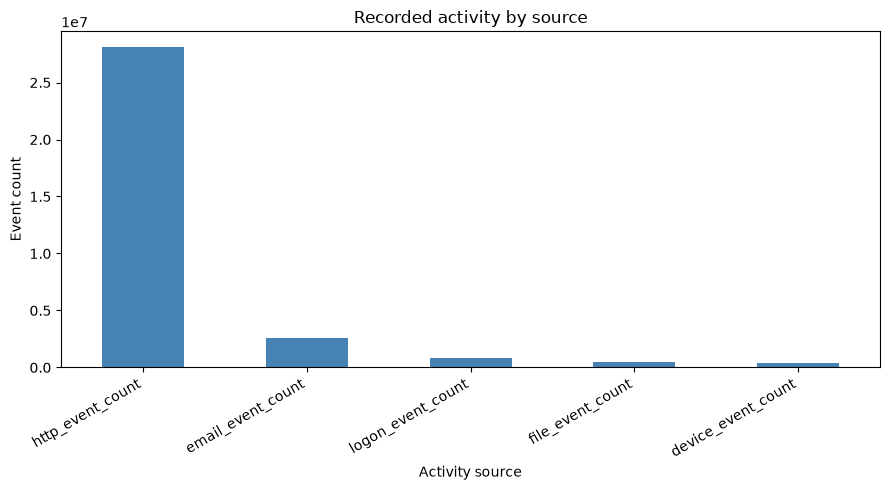
\includegraphics[width=0.79\textwidth,height=0.48\textheight,keepaspectratio]{notebook-1.png}
\caption{Retained activity events by source in the notebook analysis}
\label{fig:source-counts}
\end{figure}

\begin{figure}[H]
\centering
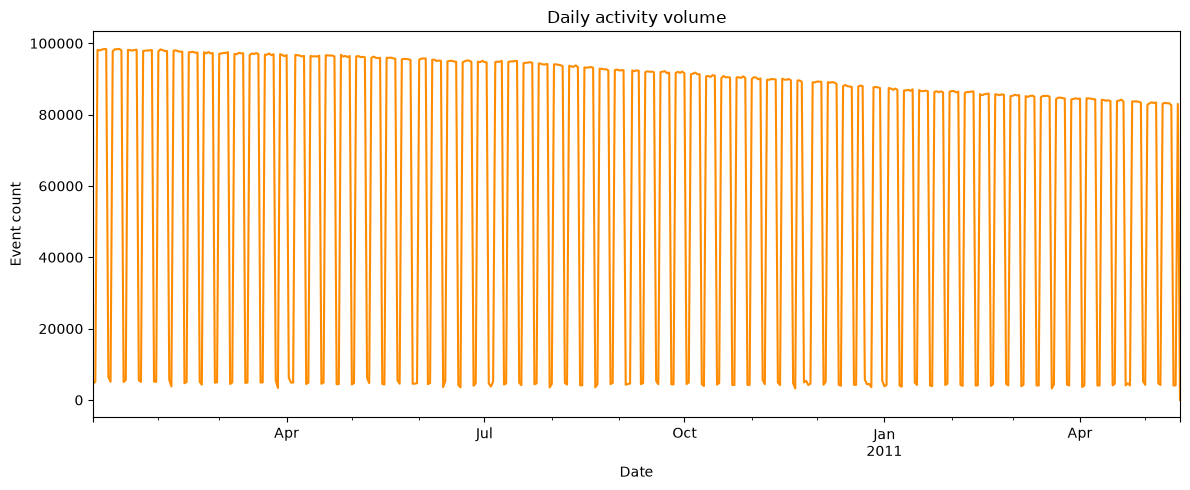
\includegraphics[width=0.9\textwidth,height=0.5\textheight,keepaspectratio]{notebook-2.png}
\caption{Daily recorded activity volume across the dataset period}
\label{fig:daily-counts}
\end{figure}

\begin{figure}[H]
\centering
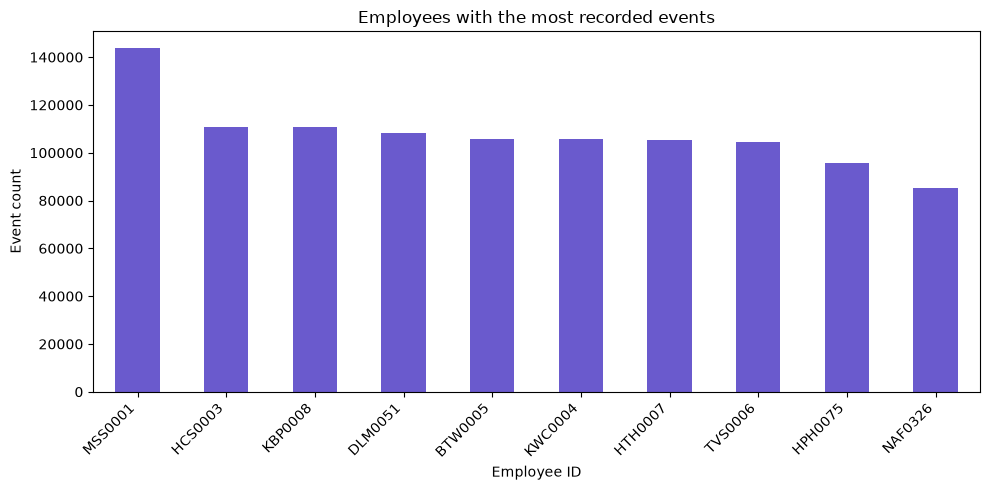
\includegraphics[width=0.83\textwidth,height=0.48\textheight,keepaspectratio]{notebook-3.png}
\caption{Ten synthetic users with the largest aggregate event counts}
\label{fig:top-users}
\end{figure}

\begin{figure}[H]
\centering
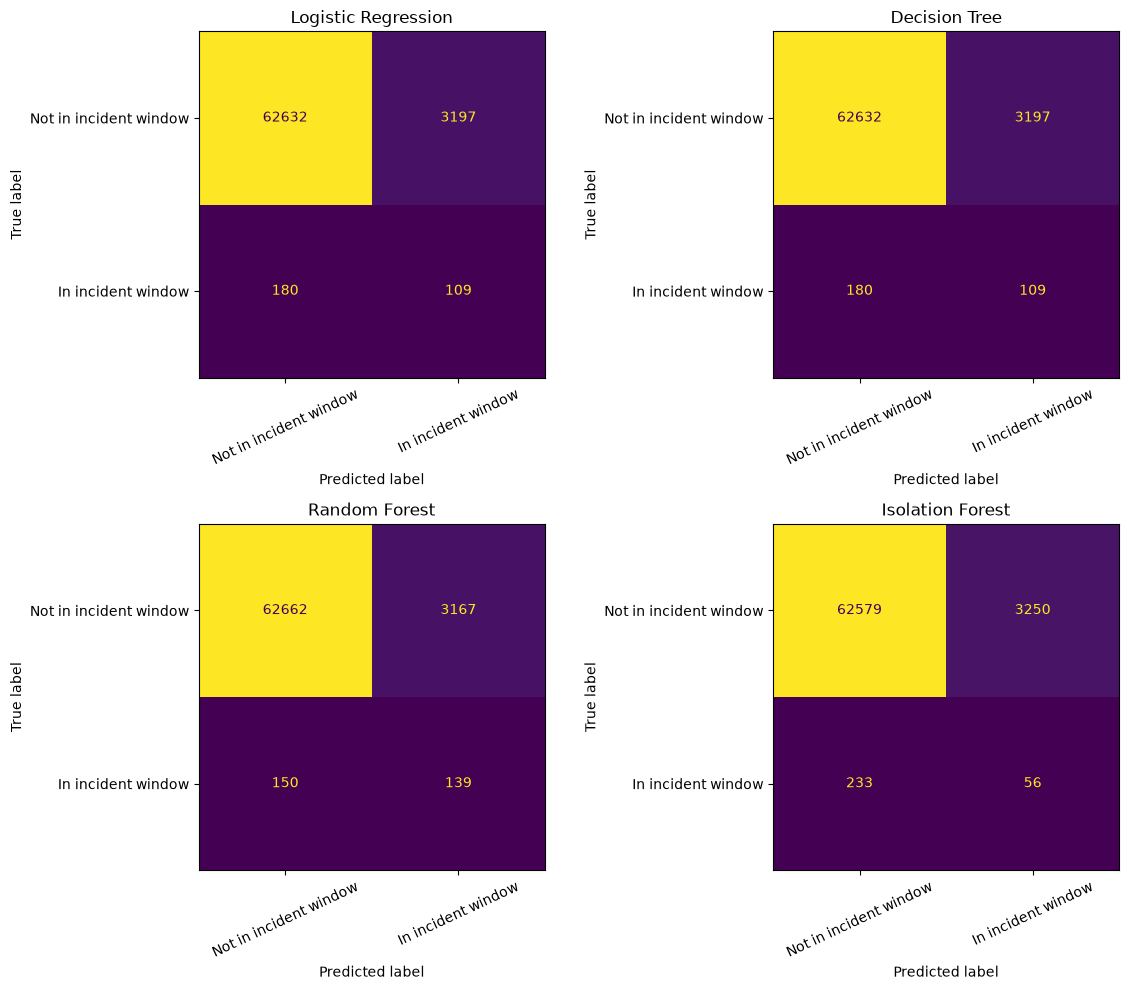
\includegraphics[width=0.85\textwidth,height=0.48\textheight,keepaspectratio]{notebook-4.png}
\caption{Model-evaluation visualization saved by the analysis notebook}
\label{fig:notebook-evaluation}
\end{figure}

The event-source plot shows why counts should be compared within an
appropriate feature and context. The daily series illustrates that
aggregate volume changes across the dataset period. The top-user chart
is not a list of suspicious employees. The evaluation visualization
must be read with the positive-class support and the review-capacity
rule; an attractive aggregate score cannot remove label uncertainty.

\section{Analysis of architecture and algorithms}

\subsection{Detailed study of the proposed algorithms}
\textbf{Logistic Regression.} The pipeline applies median imputation,
standard scaling, and a class-weighted Logistic Regression estimator.
The maximum iteration count is 1,000 and the random seed is fixed.
Scaling is important for a linear estimator when input counts have
different magnitudes. Class weighting gives the rare positive class
greater influence during fitting, but it does not by itself guarantee
high precision.

\textbf{Decision Tree.} The tree uses a maximum depth of 10, a minimum
leaf size of 10, balanced class weights, and a fixed random seed. Each
path through the tree applies feature thresholds. This can be easier to
explain than a large ensemble, but the model can still learn patterns
specific to its training data and does not provide causal explanations.

\textbf{Random Forest.} The forest contains 200 decision trees, uses a
minimum leaf size of 5, and applies
\code{balanced\_subsample} class weighting. Bootstrap variation and
aggregation can reduce the variance of an individual tree. In the
notebook, a real-data baseline is compared with an augmented candidate.
The augmented candidate is selected only when it improves validation
Average Precision. The saved comparison indicates 815 synthetic rows
were added to the selected Random Forest.

\textbf{Isolation Forest.} This model uses 200 estimators and automatic
contamination handling. It is fitted without incident labels and
assigns a lower decision function to more anomalous observations; the
pipeline reverses the sign so that larger values indicate greater
unusualness. Anomaly is not synonymous with harmful conduct, and this
model's score is not a probability.

\begin{table}[H]
\centering
\tablefont
\caption{Estimator configuration represented in the notebook}
\label{tab:model-settings}
\begin{tabularx}{\textwidth}{|p{0.23\textwidth}|p{0.33\textwidth}|Y|}
\hline
\textbf{Model} & \textbf{Configuration} & \textbf{Output used}\\\hline
Logistic Regression & Median imputation; standard scaling; class-weighted; 1,000 maximum iterations; seed 42. & Positive-class prediction score.\\\hline
Decision Tree & Maximum depth 10; minimum leaf size 10; balanced weights; seed 42. & Positive-class prediction score.\\\hline
Random Forest & 200 trees; minimum leaf size 5; balanced-subsample weights; parallel fitting; seed 42. & Positive-class prediction score; validation-selected baseline or augmented variant.\\\hline
Isolation Forest & 200 trees; automatic contamination; parallel fitting; seed 42. & Negative decision-function value, oriented so larger is more unusual.\\\hline
\end{tabularx}
\end{table}

\subsection{Step-by-step explanation of model operation}
The data flow begins with a feature matrix \(X\), binary incident-window
labels \(y\), and a user-group vector \(g\). A stratified group split
creates training, validation, and test partitions without sharing user
identifiers between them. Supervised models fit on training features
and labels. Isolation Forest fits only on training features.

For each candidate, a risk score is computed for validation data.
Random Forest compares a real-data fit to an augmented fit, where
positive training rows are resampled and count-perturbed. Validation
Average Precision selects between these variants. The notebook then
chooses a review capacity by searching candidate rates using validation
F1. Only after selection are test metrics calculated. The test set is
not used to choose the estimator or the queue rate.

\begin{enumerate}
  \item Construct and validate the employee-day feature matrix.
  \item Split groups of employees into training, validation, and test
  partitions using the notebook's stratified group splitters.
  \item Fit the four model families on training data, with labels
  supplied only to supervised models.
  \item Compare the Random Forest's baseline and augmented variants
  using validation Average Precision.
  \item Convert each score into a fixed-capacity decision for
  validation experiments and select the queue rate by validation F1.
  \item Evaluate selected estimators and operating capacity on
  untouched test data; retain both ranking metrics and confusion
  counts.
  \item Persist estimator objects, selected feature columns, and
  metadata in the model bundle for dashboard scoring.
\end{enumerate}

\subsection{Algorithm flow diagrams}
\begin{figure}[H]
\centering
\begin{tikzpicture}[
  node distance=7mm and 10mm,
  box/.style={draw,rounded corners,align=center,text width=0.68\textwidth,minimum height=8mm},
  arrow/.style={-{Stealth[length=2mm]},thick}
]
\node[box] (data) {Training employee-day features and incident-window labels};
\node[box,below=of data] (split) {Stratified group split: users are disjoint across train, validation, and test};
\node[box,below=of split] (train) {Fit model on training partition; Isolation Forest does not use labels};
\node[box,below=of train] (valid) {Score validation rows and compare candidate model variants};
\node[box,below=of valid] (select) {Select model by validation Average Precision and capacity by validation F1};
\node[box,below=of select] (test) {Evaluate once on held-out test rows and report queue metrics};
\node[box,below=of test] (save) {Save estimator bundle and feature-column contract};
\draw[arrow] (data)--(split);
\draw[arrow] (split)--(train);
\draw[arrow] (train)--(valid);
\draw[arrow] (valid)--(select);
\draw[arrow] (select)--(test);
\draw[arrow] (test)--(save);
\end{tikzpicture}
\caption{Supervised training and evaluation flow}
\label{fig:training-flow}
\end{figure}

\begin{figure}[H]
\centering
\resizebox{\textwidth}{!}{%
\begin{tikzpicture}[
  node distance=7mm and 8mm,
  box/.style={draw,rounded corners,align=center,text width=0.39\textwidth,minimum height=9mm},
  arrow/.style={-{Stealth[length=2mm]},thick}
]
\node[box] (input) {One employee-day feature row};
\node[box,below left=of input] (if) {Isolation Forest\\unusualness score};
\node[box,below right=of input] (lr) {Logistic Regression\\positive-class score};
\node[box,below=20mm of if] (dt) {Decision Tree\\positive-class score};
\node[box,below=20mm of lr] (rf) {Random Forest\\positive-class score};
\node[box,below=of dt,xshift=0.21\textwidth] (rank) {Within-batch percentile rank for each model};
\node[box,below=of rank] (mean) {Mean model rank per day; maximum day per employee};
\node[box,below=of mean] (queue) {Review status from top-five-percent consensus or two-of-four agreement};
\draw[arrow] (input)--(if);
\draw[arrow] (input)--(lr);
\draw[arrow] (input)--(dt);
\draw[arrow] (input)--(rf);
\draw[arrow] (if)--(rank);
\draw[arrow] (lr)--(rank);
\draw[arrow] (dt)--(rank);
\draw[arrow] (rf)--(rank);
\draw[arrow] (rank)--(mean);
\draw[arrow] (mean)--(queue);
\end{tikzpicture}%
}
\caption{Dashboard scoring and employee-level prioritisation}
\label{fig:ensemble-flow}
\end{figure}

The dashboard first creates percentile ranks separately within the
current scoring batch because the model outputs are on different
scales. A per-day consensus is the mean of the four ranks. The employee
table uses the highest daily consensus for each user and each model's
highest employee-level rank. The display status is set when consensus
is within the top five percent of employees or at least two model
ranks are in their respective top ten percent. This rule is intended
to prioritise review, not to classify guilt.

\section{Project pipeline}
\begin{figure}[H]
\centering
\resizebox{\textwidth}{!}{%
\begin{tikzpicture}[
  node distance=8mm and 8mm,
  stage/.style={draw,rounded corners,align=center,text width=0.29\textwidth,minimum height=15mm},
  arrow/.style={-{Stealth[length=2mm]},thick}
]
\node[stage] (input) {1. Select local folder\\Five required CSV logs};
\node[stage,right=of input] (clean) {2. Validate and clean\\Chunk reads, dates, IDs, duplicates};
\node[stage,right=of clean] (aggregate) {3. Aggregate\\Employee-day feature table};
\node[stage,below=of aggregate] (score) {4. Score\\Four saved models and percentile ranks};
\node[stage,left=of score] (review) {5. Prioritise\\Employee queue and activity detail};
\node[stage,left=of review] (export) {6. Export\\CSV summaries saved locally};
\draw[arrow] (input)--(clean);
\draw[arrow] (clean)--(aggregate);
\draw[arrow] (aggregate)--(score);
\draw[arrow] (score)--(review);
\draw[arrow] (review)--(export);
\end{tikzpicture}%
}
\caption{End-to-end project pipeline}
\label{fig:project-pipeline}
\end{figure}

\subsection{Explanation of pipeline stages}
\textbf{Input selection.} The React client gathers files from a selected
folder and posts the expected CSVs to the local API. An alternative
API endpoint accepts a folder path on the host. The application expects
the five source filenames exactly, apart from case normalisation in
upload handling.

\textbf{Validation and cleaning.} Required source presence is checked
before scoring. Each log is streamed in chunks and normalised to the
columns the aggregator needs. Missing required columns or unreadable
records cause explicit errors rather than a successful-looking empty
report.

\textbf{Aggregation and alignment.} Each source becomes a user-day
table. Tables are aligned on user and day, missing source-day
contributions are filled with zero, and the final feature matrix is
reordered to the saved feature list. This ordering is critical because
estimators bind learned parameters to column positions.

\textbf{Scoring and ranking.} Every estimator processes the same
feature matrix. Scores are converted to percentile ranks, averaged per
employee-day, and reduced to employee-level maxima. The system builds
human-readable reasons from selected high-volume signals on the
highest-consensus day.

\textbf{Review and export.} The dashboard provides a ranked queue,
summary metrics, filtering, search, per-model scores, and a short
activity table. The API and Streamlit app write day-level and
employee-level CSV outputs into \code{sprint1\_output}. The outputs are
local demonstration artifacts and are not an immutable evidence store.

\section{Feasibility analysis}

\subsection{Technical feasibility}
The system is technically feasible as a local prototype because its
components use widely available Python and JavaScript tooling, its
inputs are ordinary CSV files, and model training can be performed
offline. The scorer limits individual CSV reads to 25,000-row chunks.
The overall workflow still holds grouped and scored data in memory, so
the project has not demonstrated arbitrary-scale streaming. Runtime
and memory should be benchmarked on the target machine and data volume.

\subsection{Economic feasibility}
The software stack relies on open-source packages and a local
development environment. No hosted service, paid API, or dedicated
database is required for the demonstration. Costs remain in personnel
time, workstation resources, data governance, security review,
maintenance, and any organisational licensing or infrastructure
requirements. Open-source availability does not eliminate the cost of
operating a responsible investigation process.

\subsection{Operational feasibility}
An analyst can select a folder, run analysis, inspect a queue, and
review activity aggregates without learning the model code. The
prototype provides an understandable entry point, but it does not
support case assignment, audit trails, reviewer notes, approvals, or
incident-system integration. Operational deployment would require
those controls and a written process for challenging, documenting, and
closing a review.

\begin{table}[H]
\centering
\tablefont
\caption{Feasibility summary}
\label{tab:feasibility}
\begin{tabularx}{\textwidth}{|p{0.20\textwidth}|Y|Y|}
\hline
\textbf{Dimension} & \textbf{Current position} & \textbf{Condition for broader use}\\\hline
Technical & Local Python/API/browser stack and serialized models work as a coherent prototype. & Benchmark full data volume; add schema validation, failure recovery, and monitoring.\\\hline
Economic & No external paid service is required for the demonstration. & Budget for review staff, secure endpoints, maintenance, and governance.\\\hline
Operational & Folder selection and ranked review are straightforward. & Add case workflow, auditability, accountable reviewers, and escalation policy.\\\hline
Privacy & Feature generation omits content fields and processing is local by design. & Enforce access, retention, consent/legal basis, and secure handling of source logs.\\\hline
\end{tabularx}
\end{table}

\section{System environment}

\subsection{Software environment}
The Python backend depends on pandas, NumPy, scikit-learn, joblib,
FastAPI, Pydantic through FastAPI, python-multipart, and Uvicorn.
Streamlit is used by the alternative interface. The browser client
uses React and Vite. Exact dependency versions should be captured in a
lock file for a reproducible deployment; the repository's current
requirements file lists package names without strict versions.

\subsection{Hardware environment}
The demonstrated setup is a developer workstation capable of running
Python, a local web service, and a browser. The saved model bundle and
large data files determine the actual memory and storage requirements.
No measured minimum CPU, RAM, disk, or runtime benchmark is included in
the repository; the hardware values in Appendix 10.1 are therefore
presented as practical setup guidance, not measured guarantees.

\section{Actors and roles}
\begin{table}[H]
\centering
\tablefont
\caption{Actors and responsibilities}
\label{tab:actors}
\begin{tabularx}{\textwidth}{|p{0.22\textwidth}|p{0.36\textwidth}|Y|}
\hline
\textbf{Actor} & \textbf{Responsibilities} & \textbf{System boundary}\\\hline
Analyst / operator & Select a dataset, run analysis, inspect ranked signals, verify source evidence, document a review. & The prototype supports selection and inspection; investigation decisions remain external.\\\hline
Data custodian & Authorise use of input logs and ensure correct scope and retention. & Not implemented as an application role; required operational control.\\\hline
Model maintainer & Build and version the model bundle, record evaluation and feature schema, assess changes. & Notebook and model artifacts support development; no registry is present.\\\hline
Application operator & Start the local API and browser client, monitor errors, protect outputs. & Local developer workflow; production service controls are out of scope.\\\hline
\end{tabularx}
\end{table}

\section{Functional and non-functional requirements}
\begin{longtable}{|p{0.12\textwidth}|p{0.39\textwidth}|p{0.14\textwidth}|p{0.24\textwidth}|}
\caption{Functional and non-functional requirements}\label{tab:requirements}\\
\hline
\textbf{ID} & \textbf{Requirement} & \textbf{Class} & \textbf{Evidence in project}\\\hline
\endfirsthead
\hline
\textbf{ID} & \textbf{Requirement} & \textbf{Class} & \textbf{Evidence in project}\\\hline
\endhead
\hline
\multicolumn{4}{r}{Continued on next page}\\
\endfoot
\hline
\endlastfoot
FR-01 & Accept the five required activity sources and report missing files. & Functional & API upload validation and scorer file checks.\\\hline
FR-02 & Process records with bounded chunk reads. & Functional & Core CSV processor uses 25,000-row chunks.\\\hline
FR-03 & Reproduce the trained employee-day feature schema. & Functional & Model bundle stores \code{feature\_columns}.\\\hline
FR-04 & Score each employee-day with four estimator families. & Functional & Core scoring loop iterates through model names.\\\hline
FR-05 & Present employee-level priorities and a reason summary. & Functional & API response and dashboard queue.\\\hline
FR-06 & Show activity detail for a selected employee. & Functional & Employee endpoint returns up to 20 ranked days.\\\hline
FR-07 & Export day-level and employee-level CSV summaries. & Functional & Output files are written to \code{sprint1\_output}.\\\hline
NFR-01 & Keep the demonstration local by default. & Non-functional & API binds to loopback in the documented run configuration.\\\hline
NFR-02 & Distinguish relative ranks from probabilities or proof. & Non-functional & Dashboard text and report disclaimers.\\\hline
NFR-03 & Fail visibly when data or model prerequisites are missing. & Non-functional & API returns errors and UI displays failures.\\\hline
NFR-04 & Preserve understandable source-to-feature lineage. & Non-functional & Source-specific aggregate definitions are documented.\\\hline
NFR-05 & Support reproducible evaluation. & Non-functional & Fixed random seeds and saved evaluation artifacts.\\\hline
NFR-06 & Protect sensitive data at rest and in transit. & Non-functional & Not fully implemented; a deployment prerequisite.\\\hline
\end{longtable}
